\chapter{Температура через энтропию и энергию}

\lectureoverview{Температура сначала возникает как перевод привычных человеку термометрических единиц в микроскопические единицы энергии. После соответствующего перевода термодинамической энтропии в безразмерную статистическую энтропию мы описываем равновесие как однопараметрическое семейство распределений вероятностей. Производная \(dE/dS\) тогда определяет температуру, а первые два закона показывают, почему разность температур определяет направление потока энергии.}

\section{Коэффициенты пересчёта и единицы человеческого масштаба}

Многие физические константы служат коэффициентами пересчёта. Скорость света позволяет перевести расстояние во время:
\begin{equation}
 t=\frac{x}{c}.
\end{equation}
Если расстояния и времена измеряются в согласованных единицах, можно положить \(c=1\). Никакой физический эффект не исчезает; два вида измерения просто приведены к общей шкале.

Постоянная Больцмана имеет тот же характер. Она переводит температуру, считываемую по термометру человеческого масштаба, в энергию. Прилагательное \emph{человеческого масштаба} важно. Такие единицы выбирают потому, что макроскопические приборы могут их воспроизводить и различать, а не потому, что микроскопическая динамика выделяет именно их.

Градус Цельсия был зафиксирован делением интервала между точками замерзания и кипения воды при стандартном давлении на 100 частей. В шкале Кельвина используется градус той же величины, но нуль помещается в абсолютный нуль. Выбор другого вещества, другого интервала или градусов Фаренгейта изменил бы числа, но не физику.

\begin{classroomqa}
\audiencequestion{Разве шкала Фаренгейта не была создана ещё в XVII веке?}
\lecturerresponse{Точная дата здесь не нужна. Существенно то, что все такие шкалы конструировались вокруг температур, которые люди могли получать и измерять. Размер их градуса задаётся соглашением, а не микроскопической физикой.
\lecturetimestamp{00:01:34--00:01:50}}
\end{classroomqa}

В то время, когда создавались эти шкалы, молекулярное происхождение тепла было недоступно эксперименту. Изменение на 1 градус можно было наблюдать с помощью макроскопического термометра, тогда как энергию одной молекулы измерить было нельзя. Поэтому было естественно ввести единицу температуры прежде, чем кто-либо узнал, что по своей сути температура есть энергетическая шкала.

\section{Почему температура имеет единицы энергии}

Рассмотрим разреженный одноатомный газ. Разреженный означает, что для настоящей цели энергиями взаимодействия между молекулами можно пренебречь. В тепловом равновесии принцип равнораспределения приписывает каждой квадратичной поступательной степени свободы энергию, равную произведению постоянной Больцмана и \(T_{\mathrm K}/2\). В трёх пространственных измерениях,
\begin{equation}
 \left\langle E_{\mathrm{kin}}\right\rangle
 =\frac{3}{2}k_{\mathrm B}T_{\mathrm K}.
 \label{eq:sm2-equipartition-kelvin}
\end{equation}
Множитель 3 учитывает движение в направлениях \(x\), \(y\) и \(z\). Множитель 1/2 возникает из квадратичной кинетической энергии.

Это соотношение не ограничивается одним видом частиц. В смеси гелия и кислорода в равновесии каждая свободно перемещающаяся частица имеет одну и ту же среднюю кинетическую энергию движения центра масс, хотя более тяжёлые частицы движутся медленнее. Поскольку
\begin{equation}
 E_{\mathrm{kin}}=\frac{1}{2}mv^2,
\end{equation}
из одинаковой характерной энергии следует \(v\propto m^{-1/2}\).

Эту же идею можно довести до намеренно крайнего примера. Подвесьте шар для боулинга в текучей среде и дайте всей системе прийти к равновесию. Его броуновские поступательные степени свободы определяются той же энергетической шкалой, что и у молекулы. Скорость шара фантастически меньше, потому что его масса фантастически больше, но температура сравнивает энергетические шкалы, а не скорости.

При комнатной температуре \(T_{\mathrm K}\) составляет примерно \(300\,\mathrm K\), тогда как энергия одной микроскопической степени свободы в джоулях очень мала. Поэтому коэффициент пересчёта мал:
\begin{equation}
 k_{\mathrm B}\simeq 1.38\times10^{-23}\,
 \mathrm{J\,K^{-1}}.
 \label{eq:sm2-boltzmann-value}
\end{equation}
Его порядок величины связан с числом Авогадро, а не является случайным совпадением:
\begin{equation}
 R=N_{\mathrm A}k_{\mathrm B}.
\end{equation}
Газовая постоянная \(R\) описывает моль, тогда как \(k_{\mathrm B}\) описывает соответствующий масштаб на одну микроскопическую составляющую.

В фундаментальных формулах снова и снова встречается комбинация \(k_{\mathrm B}T_{\mathrm K}\). Поэтому удобнее определить
\begin{equation}
 T\equiv k_{\mathrm B}T_{\mathrm K}.
 \label{eq:sm2-energy-temperature}
\end{equation}
Отныне сама \(T\) имеет единицы энергии, а
\eqref{eq:sm2-equipartition-kelvin} принимает вид
\begin{equation}
 \left\langle E_{\mathrm{kin}}\right\rangle=\frac{3}{2}T.
 \label{eq:sm2-equipartition-natural}
\end{equation}
Если энергия измеряется в джоулях, то температура измеряется в джоулях. Если энергия измеряется в электрон-вольтах, то температура измеряется в электрон-вольтах. Никакой новой природной единицы, называемой единицей температуры, не существует.

\section{Два соглашения об энтропии}

Тот же перевод возникает и на стороне энтропии. Макроскопическая термодинамика выросла из анализа тепловых машин. Карно дал решающие рассуждения о тепловых машинах; Клаузиус позже ввёл термодинамическую энтропию и обозначение \(S\). В используемых здесь обозначениях назовём эту макроскопическую величину \(S_{\mathrm C}\). Её единицы — энергия, делённая на термометрическую температуру, например джоули на кельвин.

Статистическая энтропия безразмерна. Для дискретного распределения,
\begin{equation}
 S=-\sum_i p_i\log p_i.
 \label{eq:sm2-statistical-entropy}
\end{equation}
При натуральных логарифмах равновероятная бинарная альтернатива имеет энтропию \(\log2\); при логарифмах по основанию 2 та же величина называется одним битом. Эти два соглашения об энтропии связаны соотношением
\begin{equation}
 S=\frac{S_{\mathrm C}}{k_{\mathrm B}},
 \qquad
 S_{\mathrm C}=k_{\mathrm B}S.
 \label{eq:sm2-entropy-conversion}
\end{equation}
Макроскопическому значению, скромному в \(\mathrm{J\,K^{-1}}\), соответствует огромная безразмерная энтропия, потому что она подсчитывает информацию, распределённую по огромному числу микроскопических составляющих.

Уравнения \eqref{eq:sm2-energy-temperature} и
\eqref{eq:sm2-entropy-conversion} устанавливают используемое далее соглашение:
\[
 [T]=[\text{energy}],
 \qquad
 [S]=1.
\]
Теперь постоянная Больцмана может исчезнуть из рабочих формул. Её всегда можно восстановить, заменив \(T\) на \(k_{\mathrm B}T_{\mathrm K}\), а
\(S\) на \(S_{\mathrm C}/k_{\mathrm B}\).

\begin{classroomqa}
\audiencequestion{Если не считать множителя \(3/2\), не является ли новая температура просто энергией, измеряемой в джоулях?}
\lecturerresponse{Да, если в качестве единицы энергии выбраны джоули. Джоуль — это единица МКС \(\mathrm{kg\,m^2\,s^{-2}}\). Вместо этого можно использовать электрон-вольты или любую другую единицу энергии; тогда температура должна выражаться в той же единице. Множитель \(3/2\) относится к примеру идеального газа, а не к определению температуры.
\lecturetimestamp{00:15:49--00:16:45}}
\end{classroomqa}

\begin{classroomqa}
\audiencequestion{Если на доске указаны кельвины, разве \(k_{\mathrm B}\) тогда не является определённой константой?}
\lecturerresponse{Она определена после того, как заданы и единицы температуры, и единицы энергии. Замените кельвины на градусы Фаренгейта или джоули на электрон-вольты, и её численное значение изменится. Эта зависимость от единиц и есть именно поведение коэффициента пересчёта.
\lecturetimestamp{00:16:46--00:18:33}}
\end{classroomqa}

\begin{classroomqa}
\audiencequestion{Определяется ли численное значение постоянной Больцмана экспериментально?}
\lecturerresponse{Да. Исторически для её оценки требовалась микроскопическая информация об атомах и об их численной плотности. Больцман понял связь между молекулярной энергией и температурой ещё до того, как эти величины стали известны точно, примерно так же, как Ньютон понимал роль гравитационной постоянной до того, как её точно измерили.
\lecturetimestamp{00:18:46--00:20:00}}
\end{classroomqa}

\section{Равновесие — статистическое состояние}

Один лишь перевод единиц всё ещё не определяет температуру. Прикосновение к чему-то горячему даёт полезную биологическую интуицию, но температура — это производная физическая величина, построенная из энергии и энтропии.

Представьте себе систему, находящуюся в контакте с большой средой, чьи макроскопические условия фиксированы. Между ними может проходить энергия. Если у системы изначально слишком много энергии, она в среднем теряет энергию; если слишком мало, то в среднем получает её. В тепловом равновесии микроскопические обмены продолжаются, но ни в одном направлении нет среднего результирующего потока.

Пусть \(i\) обозначает точное микроскопическое состояние системы, а \(E_i\) — энергию этого состояния. Равновесие не означает, что система застывает в одном состоянии. Её взаимодействие со средой непрерывно меняет микросостояние, поэтому каждой возможности мы приписываем вероятность \(P_i\). Основные соотношения таковы:
\begin{align}
 \sum_i P_i &=1,
 \label{eq:sm2-normalization}\\
 \sum_i P_iE_i &=\overline E,
 \label{eq:sm2-mean-energy}\\
 S&=-\sum_iP_i\log P_i.
 \label{eq:sm2-equilibrium-entropy}
\end{align}
Черта над \(\overline E\) подчёркивает, что энергия подсистемы флуктуирует. Одно измерение может дать одно значение, а следующее — другое; повторные измерения приводят к распределению, среднее которого задаётся \eqref{eq:sm2-mean-energy}.

\begin{figure}[t]
\centering
\includegraphics[width=0.82\textwidth]{lecture_02_figure_02.png}
\caption{Нормировка и средняя энергия на доске: \(\sum_iP(i)=1\) и \(\sum_iP(i)E(i)=\langle E\rangle\).}
\lectureframe{00:24:10}
\end{figure}

\section{Семейство, параметризованное средней энергией}

Равновесное распределение сильно зависит от средней энергии. Поставьте кастрюлю с водой на плиту, и \(\overline E\) возрастёт; поставьте её в снег, и \(\overline E\) уменьшится. При этом меняются и вероятности. Поэтому равновесие следует рассматривать не как одно распределение, а как однопараметрическое семейство:
\begin{equation}
 P_i(\overline E).
 \label{eq:sm2-family}
\end{equation}
Каждый его член удовлетворяет
\begin{align}
 \sum_iP_i(\overline E)&=1,
 \label{eq:sm2-family-normalization}\\
 \sum_iP_i(\overline E)E_i&=\overline E.
 \label{eq:sm2-family-mean}
\end{align}

\begin{figure}[t]
\centering
\includegraphics[width=0.88\textwidth]{lecture_02_figure_03.png}
\caption{Переход к \(P(i,\overline E)\). Ранее записанные уравнения нормировки, средней энергии и энтропии остаются видимыми, пока вводится семейство распределений.}
\lectureframe{00:26:29}
\end{figure}

Для схематического графика упорядочим состояния по возрастанию \(E_i\). Тогда горизонтальную ось можно читать либо как индекс \(i\), либо как соответствующую энергию. Более высокая средняя энергия смещает вероятностный вес к состояниям, расположенным дальше вправо. Каждая кривая должна сохранять полную площадь, равную единице.

\begin{figure}[t]
\centering
\includegraphics[width=0.88\textwidth]{lecture_02_figure_04.png}
\caption{Несколько схематических распределений \(P(i,\overline E)\). Кривые, у которых вес сильнее смещен вправо, имеют большую среднюю энергию, при этом каждое распределение остается нормированным.}
\lectureframe{00:28:40}
\end{figure}

\begin{figure}[t]
\centering
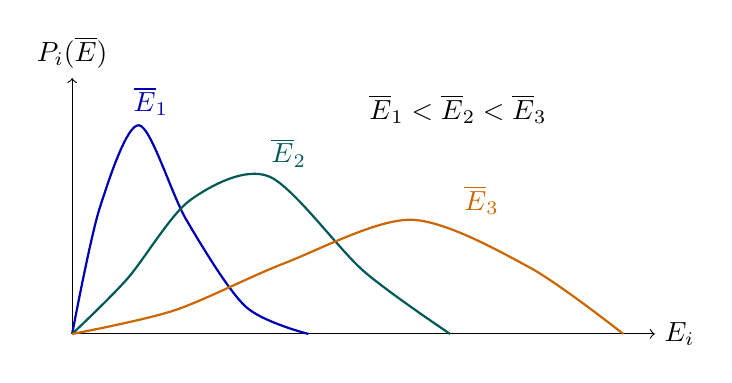
\begin{tikzpicture}[x=1cm,y=1cm]
\draw[->] (0,0) -- (7.4,0) node[right] {$E_i$};
\draw[->] (0,0) -- (0,3.25) node[above] {$P_i(\overline E)$};
\draw[thick,blue!70!black]
  plot[smooth] coordinates {(0,0) (0.35,1.6) (0.85,2.65) (1.45,1.45)
  (2.2,0.35) (3.0,0)};
\draw[thick,teal!70!black]
  plot[smooth] coordinates {(0,0) (0.7,0.7) (1.5,1.7) (2.5,2.0)
  (3.7,0.8) (4.8,0)};
\draw[thick,orange!80!black]
  plot[smooth] coordinates {(0,0) (1.3,0.3) (2.7,0.9) (4.3,1.45)
  (5.8,0.85) (7.0,0)};
\node[blue!70!black] at (1.0,2.95) {\(\overline E_1\)};
\node[teal!70!black] at (2.75,2.3) {\(\overline E_2\)};
\node[orange!80!black] at (5.2,1.7) {\(\overline E_3\)};
\node at (4.9,2.85) {\(\overline E_1<\overline E_2<\overline E_3\)};
\end{tikzpicture}
\caption{Аккуратная версия наброска на доске. Кривые не обязаны иметь именно такие точные формы; используются только нормировка и то, что их средние энергии упорядочены.}
\end{figure}

\begin{classroomqa}
\audiencequestion{Не является ли это обозначение круговым? Средняя энергия вычисляется по распределению, а распределение обозначается средней энергией.}
\lecturerresponse{Начнем с эмпирически выбранного однопараметрического семейства равновесных распределений. Каждый его член имеет среднюю энергию. Если у разных членов разные средние энергии, эту величину можно использовать как параметр семейства. Само обозначение пока не выводит это семейство; позже такой вывод даст распределение Больцмана.
\lecturetimestamp{00:28:35--00:29:44}}
\end{classroomqa}

\begin{classroomqa}
\audiencequestion{Почему говорится о средней энергии, а не о полной энергии?}
\lecturerresponse{Подсистема обменивается энергией с термостатом, например с атмосферой вокруг сосуда с газом с теплопроницаемыми стенками. Ее мгновенная энергия флуктуирует. Множество измерений дает распределение, и \(\overline E\) есть среднее этих результатов. Энергия большей замкнутой системы, состоящей из подсистемы и термостата, при этом может оставаться фиксированной.
\lecturetimestamp{00:29:46--00:30:56}}
\end{classroomqa}

\begin{classroomqa}
\audiencequestion{Могут ли разные микросостояния иметь одну и ту же энергию, и могут ли разные распределения иметь одну и ту же среднюю энергию?}
\lecturerresponse{Возможны оба варианта. Ограничение только на среднюю энергию само по себе допускает много распределений, поэтому специальное однопараметрическое равновесное семейство требует дополнительного физического аргумента. Его происхождение и больцмановская форма будут выведены позже. Равенство энергий различных микросостояний — отдельный вопрос, называемый вырожденностью.
\lecturetimestamp{00:30:58--00:32:22}}
\end{classroomqa}

\subsection{Метки состояний, вырожденность и корреляция}

Следует различать несколько понятий, которые легко смешать.

Во-первых, многие распределения вероятностей могут иметь одну и ту же среднюю энергию. Однопараметрическое равновесное семейство не получается из одного лишь ограничения на среднюю энергию. Это то конкретное семейство, которое отбирается установлением равновесия; позже будет показано, что его форма есть распределение Больцмана.

Во-вторых, несколько различных микросостояний могут иметь одну и ту же энергию. Это называется вырожденностью. В обсуждении у доски точные вырождения временно игнорируются, чтобы состояния можно было однозначно упорядочить по энергии. На деле вырожденность часто встречается, когда система обладает симметриями, но концептуальной проблемы здесь нет: сохраняйте метку состояния \(i\), допускайте повторяющиеся значения \(E_i\) и суммируйте по всем состояниям.

В-третьих, корреляция — не другое слово для вырожденности. Корреляция относится к совместному распределению двух случайных величин и спрашивает, изменяет ли знание одной из них вероятности для другой. Взаимоисключающие метки \(i\) и \(j\) в одном списке микросостояний сами по себе не являются двумя случайными величинами, корреляция которых вычисляется.

\begin{classroomqa}
\audiencequestion{Предполагает ли эта конструкция, что разные \(i\)-состояния независимы, и что, если два из них коррелированы?}
\lecturerresponse{Метка состояния — это одно из возможных значений единственной микроскопической случайной величины. Независимость и корреляция требуют двух совместно распределенных величин, поэтому такая терминология напрямую не относится к двум альтернативным меткам в этом списке. Равенство энергий разных состояний — это вместо этого вопрос о вырожденности.
\lecturetimestamp{00:32:23--00:33:22}}
\end{classroomqa}

\begin{classroomqa}
\audiencequestion{Что, если два различных состояния имеют в точности одну и ту же энергию?}
\lecturerresponse{Это и есть вырожденность. Для текущего графика мы принимаем упрощающее предположение, что никакие две энергии не совпадают, и упорядочиваем состояния по возрастанию энергии. Последующие формулы для вероятностей этого предположения не требуют; вырожденные состояния просто учитываются по отдельности.
\lecturetimestamp{00:33:23--00:34:04}}
\end{classroomqa}

\begin{classroomqa}
\audiencequestion{Произволен ли смысл индекса \(i\)?}
\lecturerresponse{Сами микроскопические состояния не произвольны: каждое задает все положения, импульсы или другие данные, необходимые для точного описания. Произвольны их названия, поэтому на рисунке мы выбираем метки в порядке возрастания энергии.
\lecturetimestamp{00:34:06--00:35:15}}
\end{classroomqa}

\section{Энтропия становится функцией энергии}

Каждый член равновесного семейства имеет энтропию. Подстановка \eqref{eq:sm2-family} в \eqref{eq:sm2-equilibrium-entropy} дает
\begin{equation}
 S(\overline E)
 =-\sum_iP_i(\overline E)\log P_i(\overline E).
 \label{eq:sm2-entropy-energy}
\end{equation}
Это не одна универсальная функция, общая для всех физических систем. Она зависит от спектра системы и от ее равновесного семейства. Однако как только это семейство задано, энергия и энтропия оказываются связаны: при переходе от одного его члена к другому меняются обе.

Обычные системы по мере роста средней энергии, как правило, распределяют вероятность между большим числом состояний, поэтому \(S\) обычно растет с \(\overline E\). Пока мы предполагаем, что эта связь гладкая и локально обратима. Исключения важны, но простой случай выявляет нужное нам определение.

\section{Производная, определяющая температуру}

Зададим конкретный вопрос: насколько должна измениться средняя энергия, чтобы увеличить энтропию на одну двоичную альтернативу? В единицах натурального логарифма такое приращение энтропии равно \(\log2\).

Для соседних членов гладкого семейства,
\begin{equation}
 dE=\frac{dE}{dS}\,dS.
 \label{eq:sm2-differential-identity}
\end{equation}
На этом этапе это уравнение — лишь правило дифференцирования сложной функции. Однако его коэффициент имеет в точности те размерности и ту физическую роль, которые требуются от температуры.

\begin{definition}
Температура в энергетических единицах определяется как
\begin{equation}
 T\equiv\frac{dE}{dS}.
 \label{eq:sm2-temperature-definition}
\end{equation}
Эквивалентно,
\begin{equation}
 dE=T\,dS,
 \qquad
 dS=\frac{1}{T}\,dE.
 \label{eq:sm2-fundamental-differentials}
\end{equation}
\end{definition}

Если изменение на один бит достаточно мало,
\begin{equation}
 \Delta E\simeq T\log2.
 \label{eq:sm2-one-bit-energy}
\end{equation}
Упор на один бит служит лишь для того, чтобы сделать производную наглядной. Любое малое изменение энтропии подчиняется тому же локальному соотношению.

\begin{classroomqa}
\audiencequestion{Раз энтропия была записана как \(S(E)\), не была бы производная \(dS/dE\) более естественной?}
\lecturerresponse{Обе производные содержат одну и ту же информацию, когда эта связь локально обратима:
\[
 \frac{dE}{dS}=\left(\frac{dS}{dE}\right)^{-1}.
\]
Температурой по принятому определению является \(dE/dS\), а обратной температурой — \(dS/dE=1/T\).
\lecturetimestamp{00:40:24--00:40:54}}
\end{classroomqa}

Здесь меняется только одна термодинамическая переменная, поэтому достаточно обычных производных. Когда допускаются изменения объема, числа частиц, намагниченности или других переменных, нужно использовать частные производные и указывать, какие величины считаются фиксированными. Настоящее определение — однопеременное сечение этой более общей термодинамической геометрии.

\subsection{Почему постоянная Больцмана сокращается}

Вернемся ненадолго к термометрическим единицам. Используя
\[
 T=k_{\mathrm B}T_{\mathrm K},
 \qquad
 S=\frac{S_{\mathrm C}}{k_{\mathrm B}},
\]
фундаментальное соотношение принимает вид
\begin{align}
 dE
 &=\bigl(k_{\mathrm B}T_{\mathrm K}\bigr)
   d\left(\frac{S_{\mathrm C}}{k_{\mathrm B}}\right)\\
 &=T_{\mathrm K}\,dS_{\mathrm C}.
 \label{eq:sm2-carnot-form}
\end{align}
Один множитель \(k_{\mathrm B}\) входит через температуру, а обратный ему множитель — через энтропию. Они сокращаются. Вот почему в обычном учебнике по термодинамике можно писать \eqref{eq:sm2-carnot-form}, не выписывая постоянную Больцмана.

\begin{classroomqa}
\audiencequestion{Должна ли \(S(E)\) быть обратимой?}
\lecturerresponse{Не всегда. Для обычных систем в рассматриваемом здесь режиме увеличение энергии обычно расширяет равновесное распределение и увеличивает энтропию, поэтому \(S(E)\) монотонна и \(T>0\). Системы с ограниченным спектром могут давать контрпримеры, включая режимы, в которых энтропия убывает с ростом энергии и статистическая температура отрицательна. Пока мы оставим эти случаи в стороне.
\lecturetimestamp{00:44:30--00:45:57}}
\end{classroomqa}

\section{От абстрактной производной к горячему и холодному}

Определение через производную универсально, но все еще абстрактно. Мы хотим восстановить привычное утверждение о том, что энергия переходит от более горячего тела к более холодному. Боль при прикосновении к горячей поверхности имеет биологическую природу; цвет и испускаемое излучение зависят от свойств света. Статистическое определение должно также иметь смысл для идеализированного газа, даже если излучением пренебречь.

\begin{classroomqa}
\audiencequestion{Может ли свет, испускаемый горячим телом, служить основным определением температуры?}
\lecturerresponse{Излучение — полезный термометр, но оно вводит физику света. Статистическая механика должна определять температуру для систем вроде ящика с газом, не опираясь на оптические свойства. Более общим критерием служит направление обмена энергией.
\lecturetimestamp{00:46:42--00:47:20}}
\end{classroomqa}

Подготовим две системы \(A\) и \(B\), каждая из которых изначально находится в собственном равновесии, с температурами \(T_A\) и \(T_B\). Сначала они изолированы друг от друга. Затем соединим их слабым тепловым контактом: \emph{тонкая трубка} позволяет небольшим количествам энергии проходить туда и обратно, не нарушая идентичности ни одной из подсистем.

\begin{figure}[t]
\centering
\includegraphics[width=0.88\textwidth]{lecture_02_figure_05.png}
\caption{Отдельно подготовленные системы \(A\) и \(B\), обозначенные температурами \(T_A\) и \(T_B\), непосредственно перед рассмотрением слабого теплового контакта.}
\lectureframe{00:48:55}
\end{figure}

\begin{figure}[t]
\centering
\begin{tikzpicture}[>=Stealth]
\draw[rounded corners,thick,fill=blue!6] (0,0) rectangle (2.6,2.4);
\draw[rounded corners,thick,fill=orange!8] (5.4,0) rectangle (8,2.4);
\draw[thick] (2.6,1.35) -- (5.4,1.35);
\draw[thick] (2.6,1.05) -- (5.4,1.05);
\draw[<->,very thick] (3.15,1.2) -- (4.85,1.2)
  node[midway,above] {\(\delta E\)};
\node at (1.3,1.45) {\Large \(A\)};
\node at (6.7,1.45) {\Large \(B\)};
\node at (1.3,0.65) {\(T_A,S_A,E_A\)};
\node at (6.7,0.65) {\(T_B,S_B,E_B\)};
\node at (4,0.35) {\small weak thermal contact};
\end{tikzpicture}
\caption{Энергия флуктуирует, проходя через слабый контакт, тогда как объединенная система остается изолированной.}
\end{figure}

Предположим, без ограничения общности,
\begin{equation}
 T_B>T_A.
 \label{eq:sm2-temperature-order}
\end{equation}
Опыт показывает, что энергия должна уходить из \(B\) и поступать в \(A\). Это ожидание превращается в расчёт благодаря трём фактам.

\subsection{Аддитивность энтропии}

Для двух слабо связанных подсистем, микроскопические альтернативы которых сочетаются независимо, число совместных возможностей перемножается:
\[
 W_{AB}=W_AW_B.
\]
Энтропия логарифмична, поэтому
\begin{equation}
 S_{\mathrm{tot}}=S_A+S_B.
 \label{eq:sm2-entropy-additivity}
\end{equation}
Тот же результат непосредственно следует из энтропии Шеннона для произведения распределений.

\begin{classroomqa}
\classquestion{Почему энтропия объединённой системы складывается?}
\lecturerresponse{Потому что лежащее в основе число альтернатив перемножается, тогда как в энтропии берётся логарифм:
\(\log(W_AW_B)=\log W_A+\log W_B\). Именно слабое взаимодействие делает возможными описание через подсистемы и этот аддитивный вид в ведущем порядке.
\lecturetimestamp{00:51:06--00:52:03}}
\end{classroomqa}

\subsection{Первое и второе начала}

Объединённая система изолирована, поэтому энергия, которой обмениваются внутри неё, сохраняется:
\begin{equation}
 dE_A+dE_B=0,
 \qquad
 dE_B=-dE_A.
 \label{eq:sm2-first-law}
\end{equation}
Это и есть первое начало в рассматриваемом эксперименте.

Второе начало здесь принимается как постулат, более глубокое объяснение которого будет дано позже.
По мере того как соединённые системы релаксируют к своему новому равновесию,
\begin{equation}
 dS_{\mathrm{tot}}=dS_A+dS_B\geq0.
 \label{eq:sm2-second-law}
\end{equation}
Строгое неравенство описывает спонтанную релаксацию вне равновесия; равенство имеет место в равновесии для обратимой вариации первого порядка.

Наконец, для каждой подсистемы справедливо определение температуры:
\begin{equation}
 dE_A=T_A\,dS_A,
 \qquad
 dE_B=T_B\,dS_B.
 \label{eq:sm2-two-temperatures}
\end{equation}

\begin{figure}[H]
\centering
\includegraphics[width=0.88\textwidth]{lecture_02_figure_06.png}
\caption{Два соотношения для подсистем \(dE_A=T_A\,dS_A\) и \(dE_B=T_B\,dS_B\) в конце вывода на доске.}
\lectureframe{00:54:00}
\end{figure}

\subsection{Знак потока энергии}

Эти уравнения уже определяют направление чистого переноса. Подставим \(dS_A=dE_A/T_A\), \(dS_B=dE_B/T_B\) и
\eqref{eq:sm2-first-law} в \eqref{eq:sm2-second-law}:
\begin{align}
 dS_{\mathrm{tot}}
 &=\frac{dE_A}{T_A}+\frac{dE_B}{T_B}\\
 &=dE_A\left(\frac{1}{T_A}-\frac{1}{T_B}\right)\geq0.
 \label{eq:sm2-flow-sign}
\end{align}
Если \(T_B>T_A>0\), то
\[
 \frac{1}{T_A}-\frac{1}{T_B}>0.
\]
Поэтому из \eqref{eq:sm2-flow-sign} следует
\[
 dE_A>0,
 \qquad
 dE_B<0.
\]
Более холодная система \(A\) получает энергию, а более горячая система \(B\) её теряет.
Когда \(T_A=T_B\), изменение энтропии первого порядка не задаёт предпочтительного
направления, и микроскопические обмены взаимно компенсируются, так что чистый перенос равен нулю. Таким образом,
абстрактная производная \(T=dE/dS\) воспроизводит операционное различие между
горячим и холодным.
